%%%%%%%%%%%%%%%%%%%%%%%%%%%%%%%%%%%%%%%%%
% FRI Data Science_report LaTeX Template
% Version 1.0 (28/1/2020)
% 
% Jure Demšar (jure.demsar@fri.uni-lj.si)
%
% Based on MicromouseSymp article template by:
% Mathias Legrand (legrand.mathias@gmail.com) 
% With extensive modifications by:
% Antonio Valente (antonio.luis.valente@gmail.com)
%
% License:
% CC BY-NC-SA 3.0 (http://creativecommons.org/licenses/by-nc-sa/3.0/)
%
%%%%%%%%%%%%%%%%%%%%%%%%%%%%%%%%%%%%%%%%%


%----------------------------------------------------------------------------------------
%	PACKAGES AND OTHER DOCUMENT CONFIGURATIONS
%----------------------------------------------------------------------------------------
\documentclass[fleqn,moreauthors,10pt]{ds_report}
\usepackage[english]{babel}

\graphicspath{{fig/}}




%----------------------------------------------------------------------------------------
%	ARTICLE INFORMATION
%----------------------------------------------------------------------------------------

% Header
\JournalInfo{FRI Data Science Project Competition 2023}

% Interim or final report
\Archive{Interim report} 
%\Archive{Final report} 

% Article title
\PaperTitle{Feature selection on large and sparse datasets} 

% Authors (student competitors) and their info
\Authors{Leon Hvastja, Amadej Pavšič}

% Advisors
\affiliation{\textit{Advisors: doc. dr. Jure Demšar, dr. Blaž Mramor, Blaž Škrlj}}

% Keywords
\Keywords{feature selection, feature ranking, machine learning, big data, sparse features ...}
\newcommand{\keywordname}{Keywords}


%----------------------------------------------------------------------------------------
%	ABSTRACT
%----------------------------------------------------------------------------------------

\Abstract{

Feature selection is a common problem in machine learning, especially when dealing with sparse datasets. In this project, we explore various out-of-the-box algorithms for feature selection, including those based on simple machine learning models and those derived from the relief algorithm. Our task is to implement, develop, and test these algorithms for smarter feature selection, enabling quicker and more efficient feature selection than using greedy algorithms. We will test the performance of our developed approaches against the optimal solution found by the greedy algorithm.

}

%----------------------------------------------------------------------------------------

\begin{document}

% Makes all text pages the same height
\flushbottom 

% Print the title and abstract box
\maketitle 

% Removes page numbering from the first page
\thispagestyle{empty} 

%----------------------------------------------------------------------------------------
%	ARTICLE CONTENTS
%----------------------------------------------------------------------------------------

\section*{Introduction}

We were given a dataset from Outbrain's regular operations which underwent minimal preprocessing tailored to our project. The company provided us with their feature scores derived using a greedy approach as a reference. Our aim is to explore if the feature selection process can be expedited while minimizing trade-offs. The project goal is to devise an intelligent approach to select features from the dataset.

We hypothesize that simple machine learning models can produce quick feature selection results, but models that account for feature interactions will be more accurate at the expense of longer computational times. Additionally, we anticipate that a heuristic feature pre-selection approach can improve processing time for complex algorithms without sacrificing scoring accuracy, which will be one of our main points of focus going forward.  

	% These latex files are intended to serve as a the template for the FRI Data Science Project Competition. If you find mistakes in the template or have problems using it, please consult Jure Demšar (\href{mailto:jure.demsar@fri.uni-lj.si}{jure.demsar@fri.uni-lj.si}).
	
	% In the Introduction section you should write about the relevance of your work (what is the purpose of the project, what will we solve) and about related work (what solutions for the problem already exist). Where appropriate, reference scientific work conducted by other researchers. For example, the work done by Demšar et al. \cite{Demsar2016BalancedMixture} is very important for our project. The abbreviation et al. is for et alia, which in latin means and others, we use this abbreviation when there are more than two authors of the work we are citing. If there are two authors (or if there is a single author) we just write down their surnames. For example, the work done by Demšar and Lebar Bajec \cite{Demsar2017LinguisticEvolution} is also important for successful completion of our project.


%------------------------------------------------

\section*{Exploratory Data Analysis}

We conducted exploratory data analysis (EDA) to gain insights into the given dataset, which was provided by Outbrain in a \textit{csv} file format. The main purpose was to familiarize ourselves with the data and start developing ideas for intelligent preprocessing. The dataset logs ad clicks and comprises over 1.5 million samples with 100 features and a binary label indicating whether the ad was clicked or not. All features are anonymized with numbered labels such as \textbf{feature0}. The data contains nominal categorical data, and all values were transformed using feature hashing making them impossible to interpret for us. There were no missing values in the dataset since these were also hashed into integers, but their specific values are unknown. 

\subsection*{Feature cardinality}
Cardinality is one of the crucial feature properties we analyzed in our EDA. We have observed that 7 features contain only one unique value, rendering them uninformative. 8 features as well as the label are binary, while 20 features have more than 1000 unique values. However, some features have very high cardinality, which may make them impractical for making predictions. Features with the highest cardinality are shown in \figurename~\ref{fig:cardinality}. 


\begin{figure}[ht]\centering 
	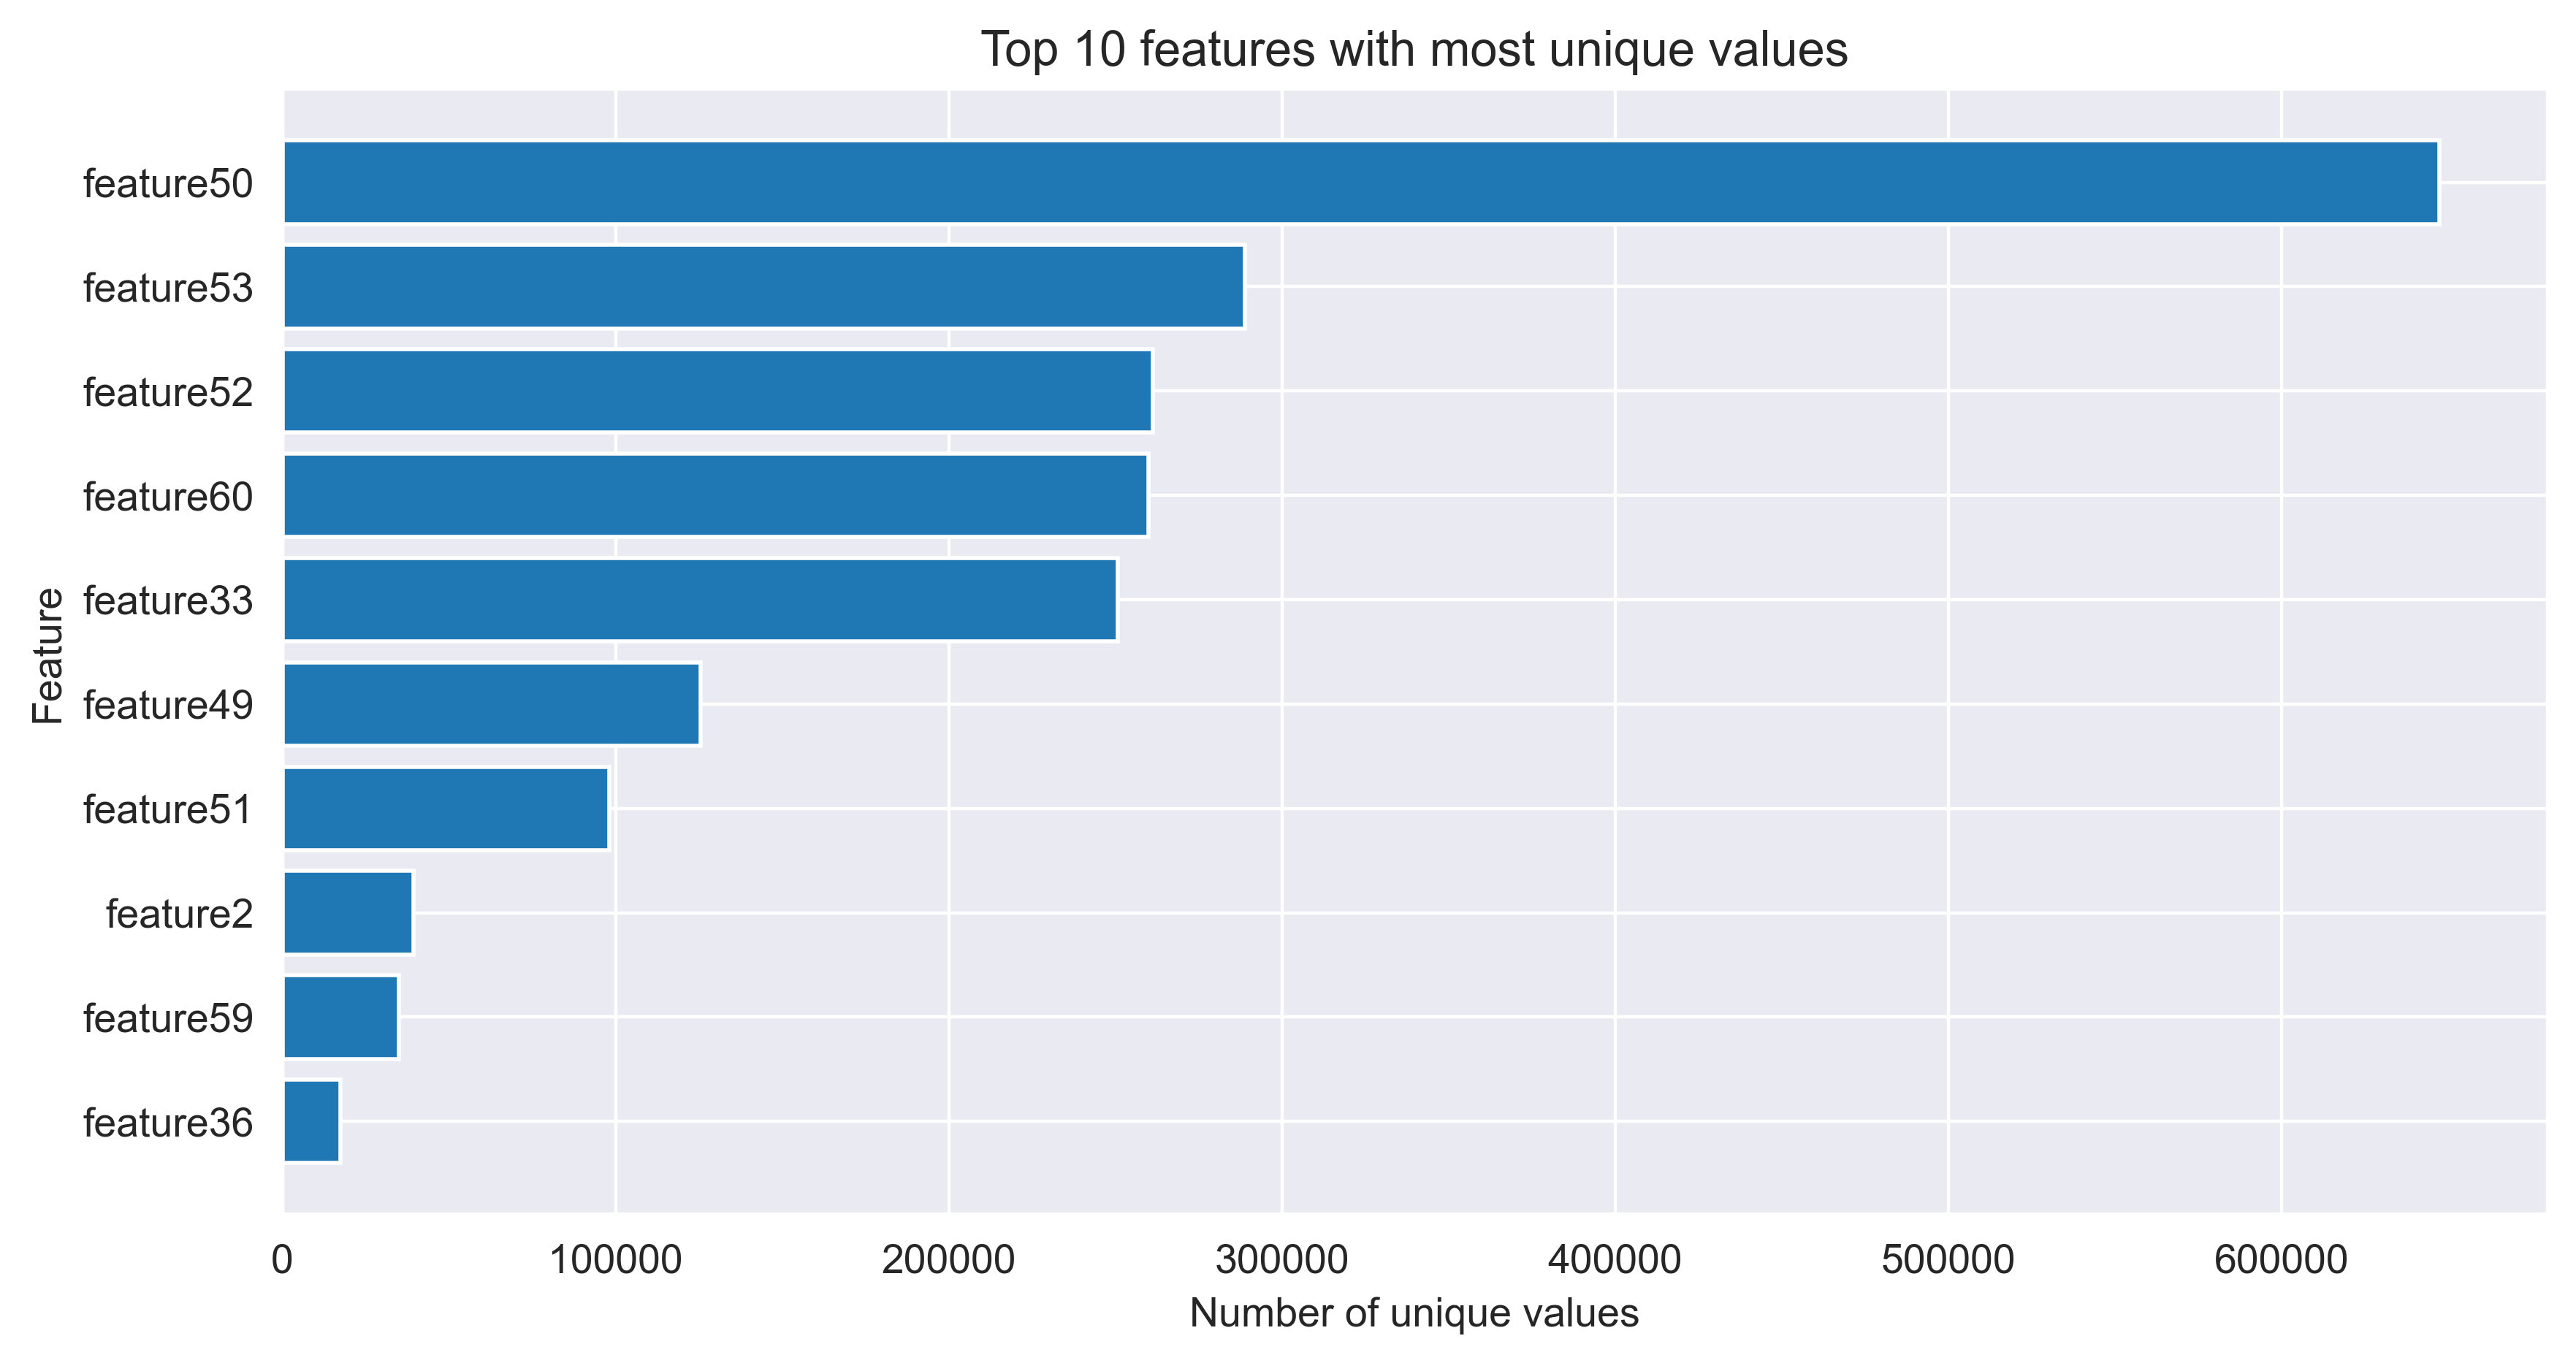
\includegraphics[width=\linewidth]{img/top10_features_unique_values.png}
	\caption{\textbf{High cardinality features.} Ten features with highest cardinality.}
	\label{fig:cardinality}
\end{figure}


\subsection*{Distribution of feature values}
The label exhibits an 80-20 ratio, indicating a bias toward the ad not being clicked. This is already a result of undersampling from the original data, which had a much higher degree of class imbalance. Additionally, the features have varying value distributions, and we observed that 13 features have one highly prevalent value, occurring in over 90\% of the samples. We inferred that these values very likely represent missing values, implying that the corresponding features are highly sparse. 

\subsection*{Feature correlation}
We utilized Pearson's coefficient (PC) to investigate the connection between characteristics and created a heatmap to demonstrate the findings. Our observations revealed a few sets of highly correlated attributes, including those ranging from 81 to 89, which are also negatively associated with the label. A dendrogram was employed to represent this clustering visually.

It's worth noting that features 98 and 99, have a perfect correlation (PC = 1) with each other and the label, effectively making them a flawless predictor of the label. These characteristics were engineered into the data, so they cannot be used for our feature selection.

\section*{Rank and Evaluation Pipeline}

We have developed a framework for evaluating features that streamlines our algorithm testing process. This pipeline handles data reading, pre-processing, feature score calculations, and evaluations against our ground truth ranking.

However, due to the large size of our dataset, one of the main challenges is managing computational complexity. Some ranking algorithms take hours to process even a small portion of the dataset, making it infeasible to apply them to the entire dataset. To tackle this issue, we plan to use our framework to run batches of evaluations on a high-power computing network. While this will allow us to perform more computations, it will not completely solve our computing complexity problem.

\subsection*{Preprocessing}
To reduce the computational load, our initial strategy involves subsampling by rows. This means selecting a random subset of data points to work with. We aim to use this approach to gain insight into the behavior of our feature scoring algorithms with larger datasets, and possibly identify an effective subsampling strategy for very large datasets. 

We also perform factorization as a preprocessing step. This involves transforming the original dataset's categories, which are represented by large integers, into a categorical form and re-encoding them as integers from 0 to n, where n represents the number of unique values for a particular feature.

\subsection*{Ranking algorithms}

There are many feature ranking algorithms and paradigms to choose from. The algorithms we chose to base our approach on fall into three categories.

\begin{enumerate}
    \item Classical approaches
    \item ML derived approaches
    \item Relief derived approaches
\end{enumerate}

The conventional methods for feature selection, such as chi-squared, Pearson correlation, ANOVA, and mutual information, fall under the category of classical approaches. They are usually quick, and their computation complexity enables us to evaluate them on the complete dataset.

The second set of approaches involves constructing a simple machine learning model on the dataset or a subset of it and deducing the implicit feature importance from the model. Most machine learning models contain some kind of implicit feature importance in the form of individual feature weights. We were interested in examining how these rankings would fare on our data. These approaches have varying time complexities.

The third category comprises algorithms based on the relief algorithm. One of the most notable characteristics of this group is that they consider feature interactions when performing the ranking. Regrettably, their time complexity is primarily quadratic, making it impractical to run on our complete dataset without significant preprocessing.

\subsection*{Ranking Evaluation}
After some experimenting with Fuzzy Jaccard \cite{Petkovic2021_fuji} score, we have together with mentors decided to stick with the simple Jaccard index for evaluating our rankings. 

We use such implementation of Jaccard, which calculates the Jaccard index for all possible "top k features". I.e. for dataset with all 100 features, we have a list of 100 Jaccard scores, and an average of them. 


% \subsection*{Code examples}

% You can also insert short code examples. You can specify them manually, or insert a whole file with code. Please avoid inserting long code snippets, advisors will have access to your repositories and can take a look at your code there. If necessary, you can use this technique to insert code (or pseudo code) of short algorithms that are crucial for the understanding of the manuscript.

% \lstset{language=Python}
% \lstset{caption={Insert code directly from a file.}}
% \lstset{label={lst:code_file}}
% \lstinputlisting[language=Python]{code/example.py}

% \lstset{language=R}
% \lstset{caption={Write the code you want to insert.}}
% \lstset{label={lst:code_direct}}
% \begin{lstlisting}
% import(dplyr)
% import(ggplot)

% ggplot(diamonds,
% 	   aes(x=carat, y=price, color=cut)) +
%   geom_point() +
%   geom_smooth()
% \end{lstlisting}

%------------------------------------------------

\section*{Results}

 Our current results have shown us the feasibility of individual algorithms. We have also identified algorithms that appear to perform poorly for our dataset regardless of undersampling rates. We've identified promising algorithms, which will now be analyzed in greater depth.

% \subsection*{More random text}

% This text is inserted only to make this template look more like a proper report. Lorem ipsum dolor sit amet, consectetur adipiscing elit. Etiam blandit dictum facilisis. Lorem ipsum dolor sit amet, consectetur adipiscing elit. Interdum et malesuada fames ac ante ipsum primis in faucibus. Etiam convallis tellus velit, quis ornare ipsum aliquam id. Maecenas tempus mauris sit amet libero elementum eleifend. Nulla nunc orci, consectetur non consequat ac, consequat non nisl. Aenean vitae dui nec ex fringilla malesuada. Proin elit libero, faucibus eget neque quis, condimentum laoreet urna. Etiam at nunc quis felis pulvinar dignissim. Phasellus turpis turpis, vestibulum eget imperdiet in, molestie eget neque. Curabitur quis ante sed nunc varius dictum non quis nisl. Donec nec lobortis velit. Ut cursus, libero efficitur dictum imperdiet, odio mi fermentum dui, id vulputate metus velit sit amet risus. Nulla vel volutpat elit. Mauris ex erat, pulvinar ac accumsan sit amet, ultrices sit amet turpis.

% Phasellus in ligula nunc. Vivamus sem lorem, malesuada sed pretium quis, varius convallis lectus. Quisque in risus nec lectus lobortis gravida non a sem. Quisque et vestibulum sem, vel mollis dolor. Nullam ante ex, scelerisque ac efficitur vel, rhoncus quis lectus. Pellentesque scelerisque efficitur purus in faucibus. Maecenas vestibulum vulputate nisl sed vestibulum. Nullam varius turpis in hendrerit posuere.

% Nulla rhoncus tortor eget ipsum commodo lacinia sit amet eu urna. Cras maximus leo mauris, ac congue eros sollicitudin ac. Integer vel erat varius, scelerisque orci eu, tristique purus. Proin id leo quis ante pharetra suscipit et non magna. Morbi in volutpat erat. Vivamus sit amet libero eu lacus pulvinar pharetra sed at felis. Vivamus non nibh a orci viverra rhoncus sit amet ullamcorper sem. Ut nec tempor dui. Aliquam convallis vitae nisi ac volutpat. Nam accumsan, erat eget faucibus commodo, ligula dui cursus nisi, at laoreet odio augue id eros. Curabitur quis tellus eget nunc ornare auctor.


%------------------------------------------------

\section*{Discussion}

To start our project, we focused on establishing baselines and evaluating various algorithms to develop a strategy for future assessments. Since our computational resources are limited, we had to narrow down our candidates. In the next phase, our attention will be on identifying the optimal feature ranking strategy for our dataset including subsampling rates, feature pre-selection and ranking algorithm choice.


%------------------------------------------------

% \section*{Acknowledgments}

% Here you can thank other persons (advisors, colleagues ...) that contributed to the successful completion of your project.


%----------------------------------------------------------------------------------------
%	REFERENCE LIST
%----------------------------------------------------------------------------------------
\bibliographystyle{unsrt}
\bibliography{report}


\end{document}